\documentclass{article}

\usepackage{amsmath, amsthm, amssymb, amsfonts}
\usepackage{thmtools}
\usepackage{graphicx}
\usepackage{setspace}
\usepackage{geometry}
\usepackage{float}
\usepackage[hidelinks]{hyperref}
\usepackage[utf8]{inputenc}
\usepackage[spanish]{babel}
\usepackage{framed}
\usepackage[dvipsnames]{xcolor}
\usepackage{tcolorbox}
\usepackage{tikz}
\usepackage{caption}
\usepackage{longtable}
\usepackage{pdflscape}
\usepackage{svg}
\usepackage{subcaption}
\usepackage{caption}
\usepackage{multirow}
\usepackage{array}
\usepackage{listings}



\begin{document}
El etiquetado de los árboles debe tener los siguientes \textit{tags}:

\begin{enumerate}
  \item \textbf{Circunferencia} (metros).
  \item \textbf{Diámetro} (milímetros).
  \item \textbf{Altura} (metros).
  \item \textbf{Diámetro de la copa} (metros).
  \item Fotos de la \textbf{corteza}, \textbf{árbol completo}, \textbf{hojas}, y, \textbf{ramas}.
\end{enumerate}

A continuación, se presenta cómo sacar estas etiquetas.

\begin{enumerate}
  \item Medir la \textbf{circunferencia} del tronco. Medir 1.30 metros desde la base del tronco y con la cinta métrica obtener la circunferencia del tronco tal como se muestra en la figura \ref{fig:circunferencia}
        \begin{figure}[H]
          \centering
          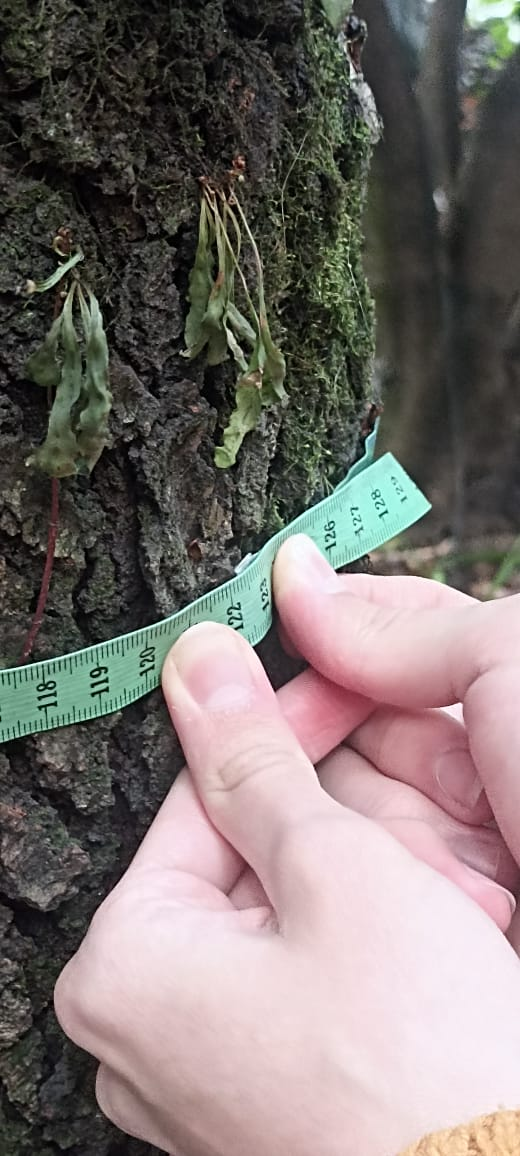
\includegraphics[width=0.3\textwidth]{img/Circunferencia.jpg}
          \caption{Obtener circunferencia del tronco}
          \label{fig:circunferencia}
        \end{figure}
  \item Se puede sacar el diámetro a partir de la circunferencia. Por eso mismo, se puede aplicar la siguiente fórmula, donde \(d\) es el diámetro, \(C\) es la circunferencia del tronco, y \(\pi\) es la constante matemática. (Recordar pasar la circunferencia de metros a milímetros multiplicando esta por 1000).
        \[
        d = \frac{C}{\pi}
        \]
  \item Se poseen dos métodos para obtener la altura de un árbol, se presentan a continuación:
        \begin{enumerate}
          \item \begin{itemize}
                  \item Para este método se requiere de un \textbf{transportador}, \textbf{cuerda}, \textbf{metro}, y, \textbf{borrador}.
                  \item Con los materiales, armar el instrumento que se presenta en la figura \ref{fig:transportador}
                        \begin{figure}[H]
                          \centering
                          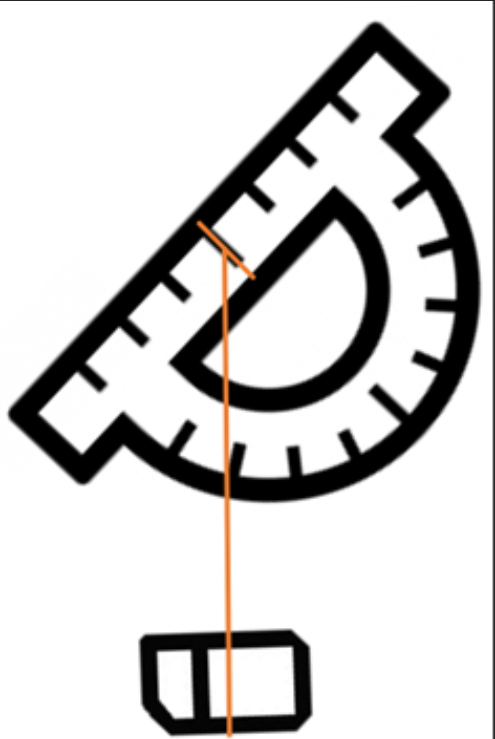
\includegraphics[width=0.3\textwidth]{img/Instrumento.png}
                          \caption{Transportador}
                          \label{fig:transportador}
                        \end{figure}
                  \item Posicionarse apuntando el transportador hacia la punta del árbol tal como se muestra en la figura \ref{fig:transportador-altura}
                        \begin{figure}[H]
                          \centering
                          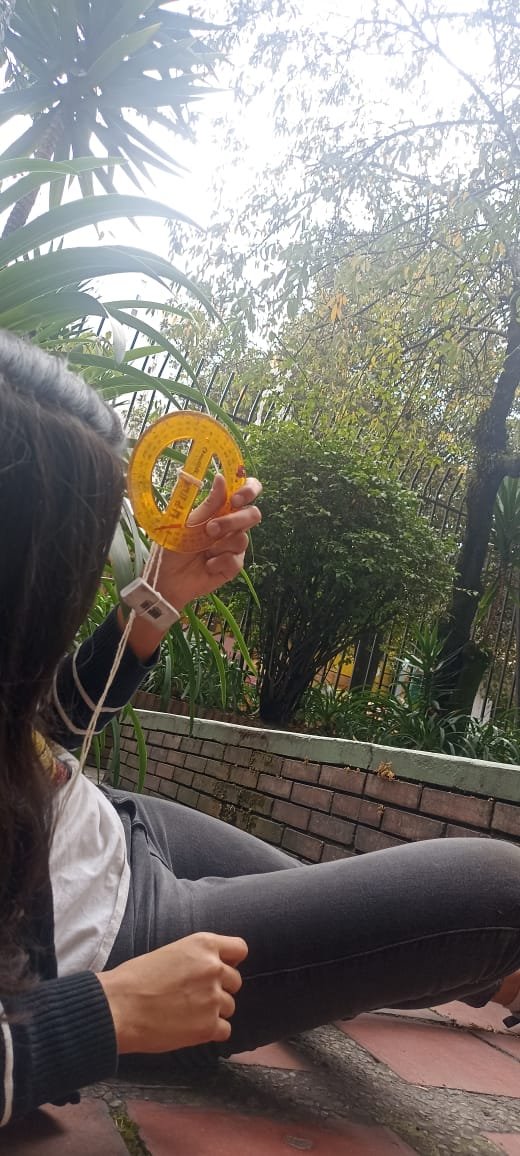
\includegraphics[width=0.2\textwidth]{img/Altura2.jpg}
                          \caption{Posición para tomar el ángulo del transportador}
                          \label{fig:transportador-altura}
                        \end{figure}
                  \item Contar cuántos grados se desplazó la cuerda desde la posición inicial y anotarlo.
                  \item Con un metro, medir cuánta distancia hay entre el árbol y la ubicación donde se obtuvó el ángulo.
                  \item Ahora, se desea hallar la altura \(h\), por lo tanto se aplicará la siguiente fórmula donde \(\theta\) es el ángulo que se obtuvo con el transportador, y, \(c\) es la distancia (en metros) que se midió con el metro. (Recordar tener la calculadora en grados).
                        \[
                        h = \tan{\theta} \times c
                        \]
                \end{itemize}
          \item Para el siguiente método se requiere; \textbf{cinta métrica} y \textbf{regla}.
                \begin{itemize}
                  \item Medir 1.30 metros desde la base del árbol y dejar una marca (cinta métrica) en dicha altura.
                  \item Alejarse hasta poder ver el árbol completo junto.
                  \item Anotar la altura del árbol completo con la regla \(h_{1}\), distancia de la base del tronco hasta la marca con la regla \(b_{1}\), tomar hasta qué distancia está la marca desde la base del tronco hasta el árbol \(b_{2}\). Realizar el siguiente cálculo para hallar la altura del árbol \(h_{2}\).
                        \[
                        h_{2} = h_{1} \times \frac{b_{2}}{b_{1}}
                        \]
                        Un ejemplo se muestra en la figura \ref{fig:altura-regla}
                        \begin{figure}[H]
                          \centering
                          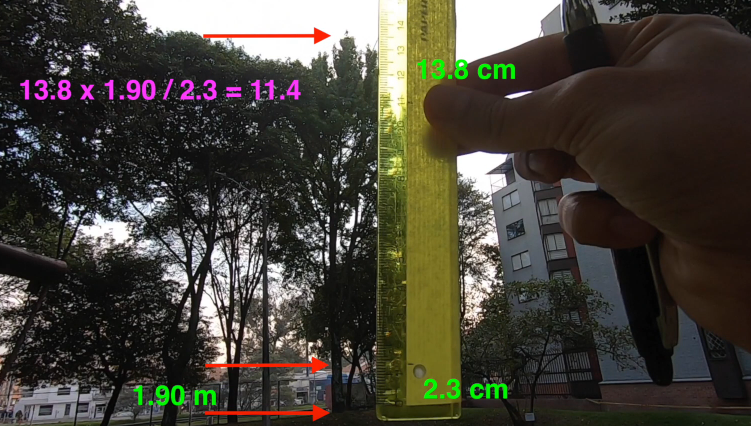
\includegraphics[width=0.8\textwidth]{img/Altura4.png}
                          \caption{Ejemplo para hallar la altura del árbol con una regla}
                          \label{fig:altura-regla}
                        \end{figure}
                \end{itemize}
          \item Realizar un promedio aritmético con ambas alturas; altura hallada con el transportador \(n_{1}\), con la regla \(n_{2}\). Entonces, la altura del árbol \(h\) será:
                \[
                h = \frac{n_{1} + n_{2}}{2}
                \]
        \end{enumerate}
  \item Para obtener el \textbf{diámetro de la copa del árbol}, se mide la distancia desde el tronco hasta la rama más lejana (figura \ref{fig:copa-arbol}) y anotar la medida en metros.
        \begin{figure}[H]
          \centering
          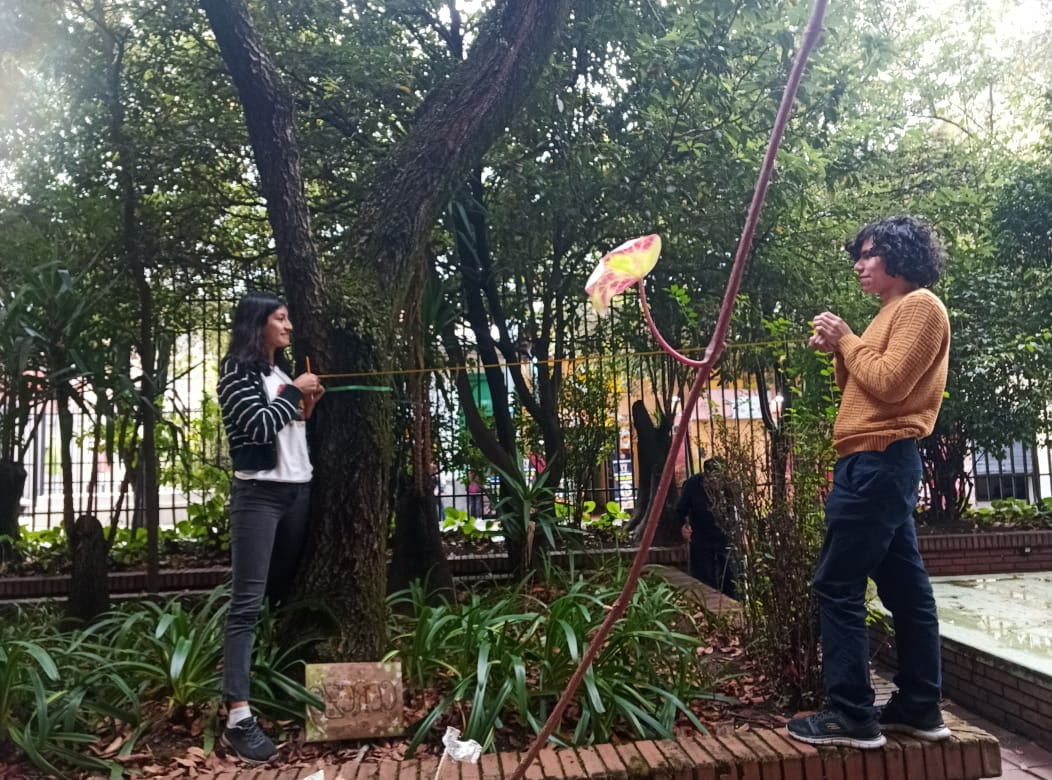
\includegraphics[width=0.8\textwidth]{img/Copa.jpg}
          \caption{Obtener la distancia de la copa del arbol}
          \label{fig:copa-arbol}
        \end{figure}

        Se ha encontrado el radio de la copa del árbol, ahora, para el diámetro \(d\) es necesario múltiplicar por 2 el radio \(r\) encontrado
        \[
        d = 2 \times r
        \]
  \item Se recomienda seguir el vídeo \url{https://www.youtube.com/watch?v=O7kSmiaFO20} para el procedimiento al momento de realizar la traza y la nota en \textit{StreetComplete}
\end{enumerate}



\end{document}
